\section{EC2}

\begin{frame}
	\frametitle{EC2}
	\begin{itemize}
		\item Oferece instâncias
		\item Podemos escolher: Processador, SO, Armazenamento, Redes, etc\dots
		\begin{figure}[htpb]
		\begin{center}
		\begin{tikzpicture}[scale=1, transform shape]
			\node at (0,0) {\huge M5d.xlarge};
			\node (M1) at (-2.3,-0.3) {};
			\node (M2) at (-1.6,-0.3) {};

			\draw (M1)--(M2);
			\draw ($(M1)!0.5!(M2)$)--($(M1)!0.5!(M2) - (0,0.2)$);
			\node at ($(M1)!0.5!(M2) - (0,0.4)$) {\tiny Family};

			\node (C1) at (-1.8,0.4) {};
			\node (C2) at (-1.2,0.4) {};

			\draw (C1)--(C2);
			\draw ($(C1)!0.5!(C2)$)--($(C1)!0.5!(C2) + (0,0.2)$);
			\node at ($(C1)!0.5!(C2) + (0,0.4)$) {\tiny Generation};

			\node (D1) at (-1.4,-0.3) {};
			\node (D2) at (-0.7,-0.3) {};

			\draw (D1)--(D2);
			\draw ($(D1)!0.5!(D2)$)--($(D1)!0.5!(D2) - (0,0.5)$);
			\node at ($(D1)!0.5!(D2) - (0,0.7)$) {\tiny Capabilities};

			\node (T1) at (-0.6,-0.3) {};
			\node (T2) at (2.3,-0.3) {};

			\draw (T1)--(T2);
			\draw ($(T1)!0.5!(T2)$)--($(T1)!0.5!(T2) - (0,0.2)$);
			\node at ($(T1)!0.5!(T2) - (0,0.4)$) {\tiny Size};
		\end{tikzpicture}
		\end{center}
		\caption{Tipo das instâncias}
		\label{fig:}
		\end{figure}
 		\item São de uso geral: Web/App servers, Gaming servers, Dev/Test Environments, etc\dots
	\end{itemize}
\end{frame}

\subsection{Tipo de instâncias}

\begin{frame}
	\frametitle{Instâncias de propósito geral}
	\begin{itemize}
		\item \textbf{Instâncias M5}: Equilíbrio entre memória, poder computacional e velocidade de rede
			\begin{itemize}
				\item Proporção de memória para vCPU é de 4:1
			\end{itemize}
		\item \textbf{Instâncias T3}: Tem uma linha base de performace da CPU e tem a possibilidade de passar a linha base (acumulando crédito ou pagando)
			\begin{itemize}
				\item Usado para workloads que não usam a CPU constantemente.
			\end{itemize}
		\item \textbf{Instâncias A1}: Workloads que precisam escalar em múltiplos cores, rodar instruções ARM, etc\dots
	\end{itemize}
\end{frame}

\begin{frame}
	\frametitle{Instâncias Memory-intensive workloads}
	\begin{itemize}
		\item Uso em: Banco de dados de alta performace, Análise de Big Data, Cache de memória, etc\dots
		\item \textbf{R5 Instances}: Workloads que processam data sets grandes em memória
			\begin{itemize}
				\item Proporção de memória para vCPU é de 8:1
			\end{itemize}
		\item \textbf{X1/X1e Instances}: Proporção de memória para vCPU é de 16:1 e 32:1
		\item \textbf{High memory instances}: Certificado para rodar SAP HANA
			\begin{itemize}
				\item Possui 6 até 24 TB de memória
			\end{itemize}
	\end{itemize}
\end{frame}

\begin{frame}
	\frametitle{Instâncias Compute-intensive workloads}
	\begin{itemize}
		\item Uso em: High-perf computing (HPC), Multiplayer Gaming, Video encoding, etc\dots
		\item \textbf{C5 Instances}: Alta performace por um preço baixo
			\begin{itemize}
				\item Proporção de memória para vCPU é 2:1
			\end{itemize}
		\item \textbf{z1d Instances}: ALta performace em uma única thread. Processador mais rápido em nuvem de 4.0 GHz
			\begin{itemize}
				\item Proporção de memória para vCPU é de 8:1
			\end{itemize}
	\end{itemize}
\end{frame}

\begin{frame}
	\frametitle{Instâncias Storage-intensive workloads}
	\begin{itemize}
		\item Uso em:
			\begin{itemize}
				\item Alta operações de I/O. Ex: High-perf databases, No SQL databases, etc\dots
				\item Muito armazenamento. Ex: Big Data, Kafka, Log processing\dots
			\end{itemize}
		\item \textbf{Instâncias I3/I3en}: Otimizadas para operações de I/O com pouca latência
		\item \textbf{Instâncias D2}: Custo baixo por armazenamento e suporta alta taxas de transferências
		\item \textbf{Instâncias H1}: Aplicações de custo baixo que usam altas transferências de dados e acesso sequencial para grandes Data Sets.
			\begin{itemize}
				\item Mais vCPUS e memória por TB que o D2
			\end{itemize}
	\end{itemize}
\end{frame}

\begin{frame}
	\frametitle{Workloads de computação acelerada}
	\begin{itemize}
		\item Uso em: Machine learning, HPC, Gráficos, etc\dots)
		\hfill
			\begin{figure}[htpb]
				\centering
				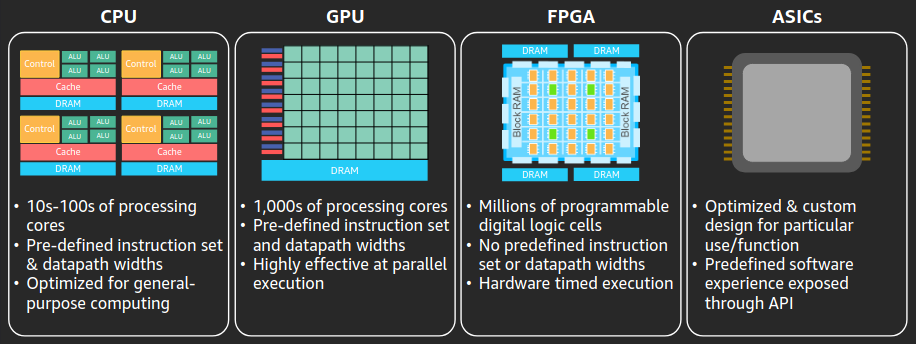
\includegraphics[width=0.8\textwidth]{ec2-comp-acc}
				\caption{CPU vs GPU vs FPGA vs ASCIs\cite{CDOLR}}
			\end{figure}
	\end{itemize}
\end{frame}

\begin{frame}
	\frametitle{Instâncias de computação acelerada}
	\begin{itemize}
		\item \textbf{Instâncias P2/P3}: GPU (deep learning training, HPC, etc\dots)
		\item \textbf{Instâncias G3/G4}: GPU (renderização 3D, codificação de vídeo, etc\dots)
		\item \textbf{Instâncias F1}: FPGAs programáveis (processamento de imagem, computação financeira, etc\dots)
		\item \textbf{Instâncias Inf1}: Alta performace e custo baixo para machine learning
			\begin{itemize}
				\item Integração com ML frameworks (TensorFlow, PyTorch, etc\dots)
			\end{itemize}
	\end{itemize}
\end{frame}

\begin{frame}
	\frametitle{Instâncias Bare Metal}
	\begin{itemize}
		\item Feito para workloads que não são virtualizados ou precisam de tipos específicos de hypervisors ou tem licenças que restrigem o uso de virtualização
	\end{itemize}
\end{frame}

\subsection{Amazon Machine Image (AMI)}

\begin{frame}
	\frametitle{Amazon Machine Images (AMIs)}
	\begin{itemize}
		\item Amazon Maintained
			\begin{itemize}
				\item Imagens de Windows e Linux
				\item Recebem Updates pela amazon em cada região
				\item Amazon Linux 2 (5 anos de suporte)
			\end{itemize}
		\item Marketplace Maintained
			\begin{itemize}
				\item São gerenciados e mantidos pelos parceiros da AWS
			\end{itemize}
		\item Your Machine Images
			\begin{itemize}
				\item AMIs que foram criadas de instâncias EC2
				\item Podem ser privadas, compartilhadas com outras contas ou publicadas na comunidade
			\end{itemize}
	\end{itemize}
\end{frame}

\subsection{EBS}

\begin{frame}
	\frametitle{Amazon EBS}
	\begin{itemize}
		\item Blocos de armazenamento como serviço
		\item Escolher o armazenamento e computar baseado no seu workload
		\item Pode colocar ou retirar de uma instância
		\item Volumes magnéticos ou baseados em SSD
		\item Suportam snapshots de um bloco modificado
		\item Dados criptografados por padrão em volumes EBS
		\item Fast Snapshot Restore (FSR)
		\item Rede mais otimizada para EBS em instâncias C5/C5d, M5/M5d, R5/R5d
	\end{itemize}
\end{frame}

\subsection{Security Group}

\begin{frame}
	\frametitle{Security Group}
	\begin{itemize}
		\item Firwall virtual para controlar a entrada e saída de tráfego em instâncias EC2
	\end{itemize}
\end{frame}

\subsection{Autoscaling groups}

\begin{frame}
	\frametitle{Autoscaling groups}
	\begin{itemize}
		\item Permite escalar horizontalmente as instâncias EC2
		\item O amazon EC2 auto scaling garante que o seu grupo vai ter a quantidade desejada de instâncias
		\item É possível configurar o Auto Scaling group para aumentar a capacidade em um dia e horário específico
		\item O dynamic scaling define como escalar os recursos dependendo da mudança da demanda
		\item É possível usar o CloudWatch para aumentar o número de servers usando algum parâmetro definido
		\item Health checks
	\end{itemize}
\end{frame}

\subsection{Elastic IP}

\subsection{Load Balancers}

\begin{frame}
	\frametitle{Classic Load Balancer}
	\begin{itemize}
		\item Suporte para EC2-Classic
		\item Suporte para TCP e SSL
		\item Suporte para sticky sessions usando cookies gerados pela aplicação
		\item Redireciona as requisições para instâncias registradas
		\item Tem health-checks
	\end{itemize}
\end{frame}

\begin{frame}
	\frametitle{Application Load Balancer}
	\begin{itemize}
		\item Funciona na camada de aplicação do modelo OSI (HTTP, HTTPS, gRPC)
		\item É possível adicionar regras para poder redirectionar as requisições de forma mais precisa
		\item Health checks podem ser feitos em grupos de instâncias
		\item Benefícios em relação ao clb:
			\begin{itemize}
				\item Path conditions (URL)
				\item Host conditions (Host field in http header)
				\item HTTP header conditions
				\item Multiplas aplicações em um EC2 (Bom para mircoserviços)
			\end{itemize}
	\end{itemize}
\end{frame}

\begin{frame}
	\frametitle{Netowrk Load Balancer}
	\begin{itemize}
		\item Funciona na camada de rede (TCP, UDP, TLS)
		\item Foward TCP traffic
		\item High performance
		\item Support static / Elastic IP
		\item Latency 100 ms (400 ms ALB)
	\end{itemize}
\end{frame}

\begin{frame}
	\frametitle{Gateway Load Balancer}
	\begin{itemize}
		\item Gateway + Load Balancer
			\begin{itemize}
				\item Next-hop in route table
				\item NO packet rewrite
			\end{itemize}
		\item Layer 3 load balancer
			\begin{itemize}
				\item Provide horizontal scale to appliances
				\item Fault tolerance for appliances
				\item Insert services transparently
				\item Share across differente VPCs and accounts
				\item Provide appliance as a service
			\end{itemize}
		\item get package of IP and use to part of appliance
		\item Thirt party appliance
		\item Simplify applicance deployment
		\item Conectar VPCs diferentes:
			\begin{itemize}
				\item Fazer appliance ou segurança
			\end{itemize}
	\end{itemize}
\end{frame}

\begin{frame}
	\frametitle{Comparação}
	\begin{table}[htpb]
		\centering
		\caption{Fonte\footnote{\href{https://aws.amazon.com/pt/elasticloadbalancing/features/\#Product_comparisons}{Comparação dos load balancers}}}
	
		\begin{tabular}{|c|c|}
			\hline
			a & a \\
			\hline \hline
		\end{tabular}
	\end{table}
\end{frame}
